\documentclass[12pt, a4paper]{article}

% Text languages
\usepackage[english, UKenglish, USenglish, american, british]{babel}

% Accents
%usepackage[latin1]{inputenc}

% Maths
\usepackage{mathtools}
\usepackage{amsmath,amsthm,amssymb}

% Double rows
%\usepackage{multirow}

% Math-mode symbol & verbatim
%\def\W#1#2{$#1{#2}$ &\tt\string#1\string{#2\string}}
%\def\X#1{$#1$ &\tt\string#1}
%\def\Y#1{$\big#1$ &\tt\string#1}
%\def\Z#1{\tt\string#1}

% A non-floating table environment.
%\makeatletter
%\renewenvironment{table}%
%   {\vskip\intextsep\parskip\z@
%    \vbox\bgroup\centering\def\@captype{table}}%
%   {\egroup\vskip\intextsep}
%\makeatother

%\DeclarePairedDelimiter\abs{\lvert}{\rvert}%
%\DeclarePairedDelimiter\norm{\lVert}{\rVert}%

% Swap the definition of \abs* and \norm*, so that \abs
% and \norm resizes the size of the brackets, and the 
% starred version does not.
%\makeatletter
%\let\oldabs\abs
%\def\abs{\@ifstar{\oldabs}{\oldabs*}}
%
%\let\oldnorm\norm
%\def\norm{\@ifstar{\oldnorm}{\oldnorm*}}
%\makeatother

% C++
\usepackage{listings}
\usepackage{xcolor}
\lstset { %
	language = C++,
	backgroundcolor=\color{black!5}, % set backgroundcolor
    basicstyle=\footnotesize,% basic font setting
    tabsize=4, % tab space width
    showstringspaces=false, % don't mark spaces in strings
    %numbers=left, % display line numbers on the left
    commentstyle=\color{green}, % comment color
    keywordstyle=\color{blue}, % keyword color
    stringstyle=\color{red} % string color
}

% https://www.overleaf.com/learn/latex/Page_size_and_margins
\usepackage{geometry}
\topmargin = -23pt
\oddsidemargin = 13pt
\headheight = 12pt
\headsep = 25pt
\textheight = 674pt
\textwidth = 426pt
\marginparsep = 10pt
\marginparwidth = 50pt
\footskip = 30pt
\marginparpush = 5pt
\hoffset = 0pt
\voffset = 0pt
\paperwidth = 597pt
\paperheight = 845pt

% Hyperlinks
\usepackage{hyperref}

% Figure
\usepackage{graphicx}
\usepackage{caption}
\usepackage{subcaption}
\usepackage{etoc}
% Example
\newtheorem{exmp}{Example}[section]
% Algorithms
%\usepackage[]{algorithm2e}
%\usepackage{algorithm}% http://ctan.org/pkg/algorithm
%\usepackage{algpseudocode}% http://ctan.org/pkg/algorithmicx
\usepackage{algpseudocode}

\renewcommand{\thefootnote}{\arabic{footnote}} % 1, 2, 3... (la que hay por defecto)

%\usepackage{titlesec}
%\setcounter{secnumdepth}{5}

%\titleformat{\paragraph}
%{\normalfont\normalsize\bfseries}{\theparagraph}{1em}{}
%\titlespacing*{\paragraph}
%{0pt}{3.25ex plus 1ex minus .2ex}{1.5ex plus .2ex}

\usepackage{float}
%--------------------------------------------------------------------------
\title{PARALLELISM}
\author{Roger Vilaseca Darné and Xavier Martín Ballesteros\\
  \small UNIVERSITAT POLITÈCNICA DE CATALUNYA\\
}
\date{10th December 2018}

\begin{document}
% Images
\graphicspath{ {./images} }

%\maketitle

\begin{titlepage}
	\centering
%	{\scshape\LARGE UNIVERSITAT POLITÈCNICA DE CATALUNYA \par}
	\vspace{1cm}
	{\scshape\Large UNIVERSITAT POLITECNICA DE CATALUNYA\par}
	\vspace{1.5cm}
	{\huge\bfseries PARALLELISM\par}
	\vspace{2cm}
	{\Large\itshape \textbf{Lab 2: Brief tutorial on OpenMP programming model}\par}
	\vfill
	{\Large\itshape Roger Vilaseca Darne and Xavier Martin Ballesteros\break PAR4110\par}
	\vfill
%	
\includegraphics[width=0.25\textwidth]{./images/UPC.png}\par\vspace{1cm}
	%supervised by\par
	%Dr.~Mark \textsc{Brown}

	\vfill

% Bottom of the page
	{\large 20th March 2019, Q1}
\end{titlepage}

%\abstract{Esto es una plantilla simple para un articulo en \LaTeX.}

%	*********************** ÍNDEX *********************
\setcounter{secnumdepth}{5}

\newpage
  \tableofcontents
\newpage

% Referència a una equació \ref{eq:area}).
% Referència a una secció \ref{sec:nada}
% Referència a una cita \cite{Cd94}.

\section{Introduction}

Talk about the Mandelbrot Set and about what we are going to do in this 3 sessions, in order.

\section{Task decomposition analysis with \textit{Tareador}}

In this section, we had to analyse the two possible task granularities that could be exploited in the given program. To do it, we used the \textit{Tareador} tool, which was very useful to see graphically the created tasks and which dependences are between them.

\subsection{Point decomposition}

In this decomposition strategy, a task corresponds with the computation of a single point (row, col) of the Mandelbrot set. Thus, we will have $row \times col$ tasks.

In order to analyse the potential parallelism of this strategy, we modified the code in \textit{mandel-tar.c} to create several \textit{Tareador} tasks. As we are using a point decomposition strategy, the tasks are created inside the most inner loop of the function mandelbrot.  Figure \ref{code:mandeltarPoint} shows the fragment of the function that we modified.

\begin{figure}[H]
\begin{lstlisting}
for (row = 0; row < height; ++row) {
	for (col = 0; col < width; ++col) {
		tareador_start_task("point");
		
		...
		
		tareador_end_task("point");
	}
}
\end{lstlisting}
\caption{Modified fragment of the \textit{mandel-tar.c} code.}
\label{code:mandeltarPoint}
\end{figure}

Once we did this, we executed interactively mandeld-tar and mandel-tar using run-tareador.sh script. The first one is used for timing purposes and to check for the numerical validity of the output (-o option) whereas with the second one we can visualize the Mandelbrot set.

The script has defined inside the size of the image to compute (-w option). In this case, the value was 8 to generate a reasonable task graph in a reasonable execution time. Hence, as we said before, the number of tasks will be $8 \times 8 = 64$.

Figures \ref{fig:mandel-tar-point} and \ref{fig:mandeld-tar-point} below show the two task decomposition graphs (TDG) of the two possible executions. There are some nodes bigger than the others. This is because these nodes have executed more instructions than the rest. Therefore, these nodes represent pixels in white\footnote{The bigger the node, the more iterations it does in the do while fragment of the function. This make that the computed color is white.}.

\begin{figure}[H]
	\centering
	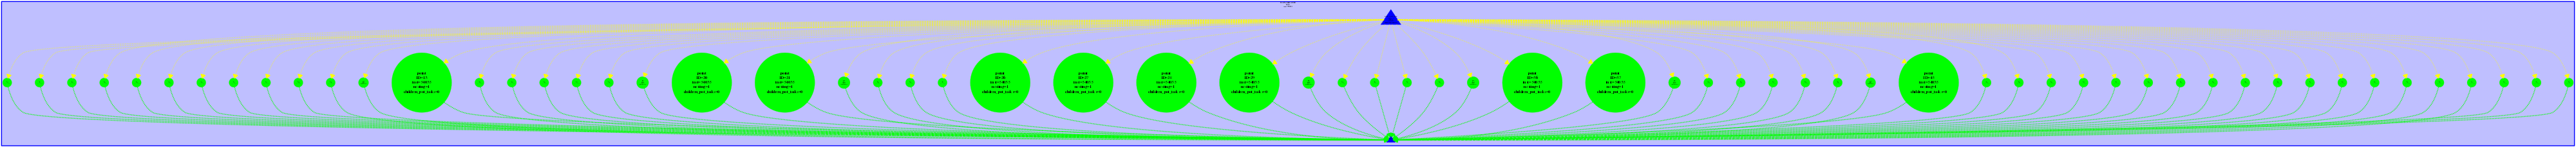
\includegraphics[scale=0.106]{./mandel-tar_point}
	\caption{Mandel-tar task decomposition graph using the point decomposition strategy.}
	\label{fig:mandel-tar-point}
\end{figure}

\begin{figure}[H]
	\centering
	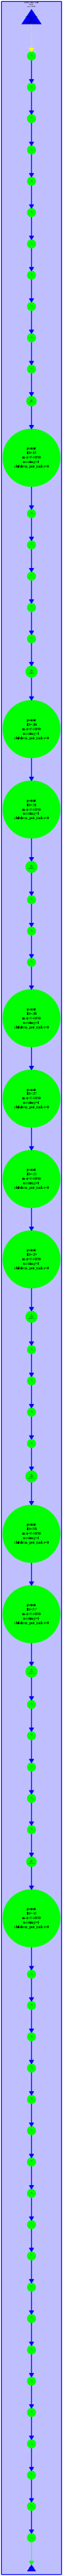
\includegraphics[scale=0.106]{./mandeld-tar_point}
	\caption{Mandeld-tar task decomposition graph using the point decomposition strategy.}
	\label{fig:mandeld-tar-point}
\end{figure}

This strategy will have more overhead of creation and termination of tasks than in the row strategy because it has to create more tasks. However, as a positive point the tasks are better distributed because if in a row there are many white areas, this work will not only be done by a single thread. Thus, it may end the execution earlier than in the row decomposition strategy.

\subsection{Row decomposition}

In this other strategy, a task corresponds with the computation of a whole row of the Mandelbrot set. This strategy only creates $row$ tasks.

In this case, the code is not the same as before. We changed the creation of the \textit{Tareador} tasks so that each time we enter a new row (second loop) a new task is created. The modified version of the code is shown below.

\begin{figure}[H]
\begin{lstlisting}
for (row = 0; row < height; ++row) {
	tareador_start_task("row");
	for (col = 0; col < width; ++col) {
		...
	}
	tareador_end_task("row");
}
\end{lstlisting}
\caption{Modified fragment of the \textit{mandel-tar.c} code.}
\label{code:mandeltarRow}
\end{figure}

Afterwards, we executed interactively mandel-tar and mandeld-tar again. We used the same size as before. Hence, the total number of tasks will be 8. The graphical results we got can be seen in figures \ref{fig:mandel-tar-row} and \ref{fig:mandeld-tar-row}.

\begin{figure}[H]
	\centering
	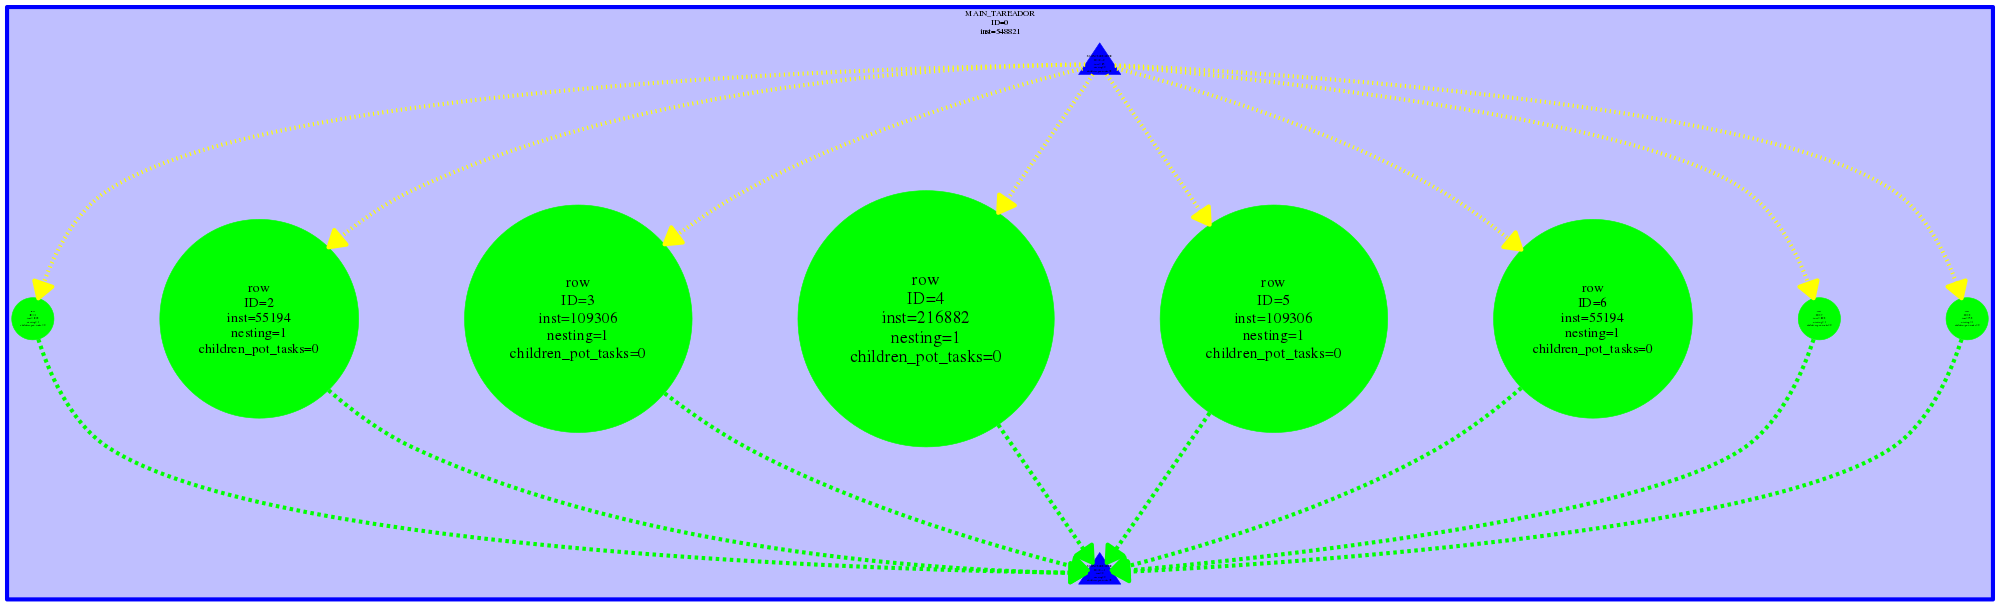
\includegraphics[scale=0.106]{./mandel-tar_row}
	\caption{Mandel-tar task decomposition graph using the row decomposition strategy.}
	\label{fig:mandel-tar-row}
\end{figure}

\begin{figure}[H]
	\centering
	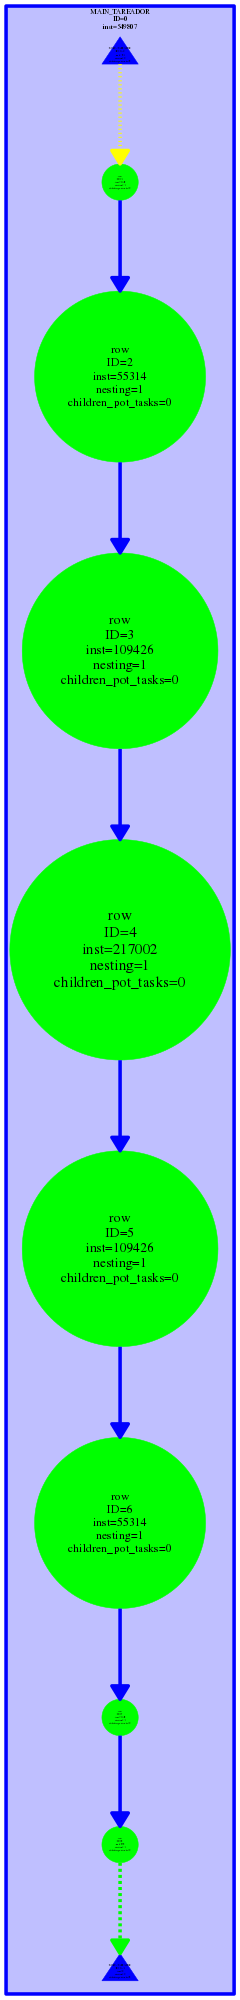
\includegraphics[scale=0.106]{./mandeld-tar_row}
	\caption{Mandeld-tar task decomposition graph using the row decomposition strategy.}
	\label{fig:mandeld-tar-row}
\end{figure}

In this strategy, the overhead time of creation and termination of tasks will be very small in comparison with the point strategy because it has to create less tasks. Nevertheless, it may happen that in a full row, all of its pixels must be white. In this case, it can happen that while other threads have finished their work, this other thread is still executing the row. Consequently, it is possible that the execution time may be bigger than in the point decomposition strategy.

\subsection{Characteristics of the TDG}

We saw in the previous sections that the execution of the mandel-tar has a very different task dependence graph than the execution of the mandeld-tar.

On the one hand, we can see that in mandel-tar every point is independent from the others. Consequently, we could parallelize that fragment of the code using OpenMP clauses.

On the other hand, in mandeld-tar we can see that all iterations have became sequential. In this situation, we do not gain anything by parallelizing the code, but we increase the execution time because of the overhead of creation and termination of tasks.

Using the \textit{Tareador} we could see which variable was responsible of creating those dependences. We did the following: Right Click into a task -$>$ Data View -$>$ Edges-out -$>$ Real Dependency. Figure \ref{fig:dependence_X11_COLOR_fake} shows the result we got.

\begin{figure}[H]
	\centering
	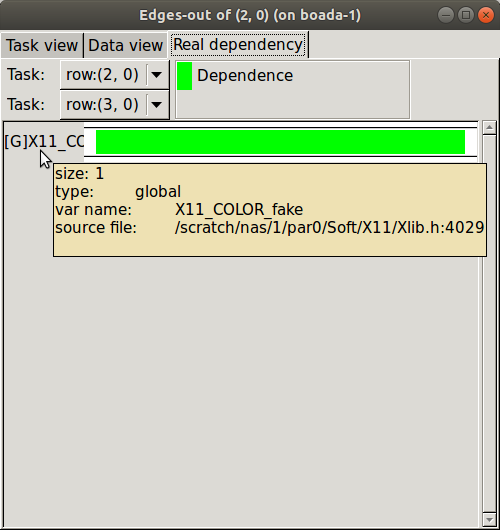
\includegraphics[scale=0.5]{./dependence_X11_COLOR_fake}
	\caption{Variable that provoques the dependences between tasks.}
	\label{fig:dependence_X11_COLOR_fake}
\end{figure}

We can see that there is only one variable that is causing all the dependences: X11\_COLOR\_fake. Observing the code, we noticed that the only difference between mandel-tar and mandeld-tar was a fragment of the code that was only executed in mode \_DISPLAY\_ (mandeld-tar):

\begin{figure}[H]
\begin{lstlisting}
#if _DISPLAY_
    /* Scale color and display point  */
    long color = (long) ((k-1) * scale_color) + min_color;
    if (setup_return == EXIT_SUCCESS) {
        XSetForeground (display, gc, color);
        XDrawPoint (display, win, gc, col, row);
    }
#else
    output[row][col]=k;
#endif
\end{lstlisting}
\caption{Fragment of the \textit{mandel-tar.c} code.}
\label{fig:display_code}
\end{figure}

Therefore, variable X11\_COLOR\_fake is used at least in one of the functions XSetForeground and XDrawPoint. We could protect this section of code in the parallel OpenMP code using the \textit{critical} clause to define a region of mutual exclusion where only one thread can be working at the same time.

\begin{figure}[H]
\begin{lstlisting}
#if _DISPLAY_
    /* Scale color and display point  */
    long color = (long) ((k-1) * scale_color) + min_color;
    
    #pragma omp critical
    if (setup_return == EXIT_SUCCESS) {
        XSetForeground (display, gc, color);
        XDrawPoint (display, win, gc, col, row);
    }
#else
    output[row][col]=k;
#endif
\end{lstlisting}
\caption{Fragment of the \textit{mandel-tar.c} code using the \textit{critical} clause to protect a fragment of the code.}
\label{fig:display_code}
\end{figure}

\end{document}
